\documentclass[12pt]{article}

\usepackage[margin=1in]{geometry}
\usepackage{amsmath,amsthm,amssymb,graphicx,gensymb,multicol,mathtools}
\usepackage{color}
\usepackage[english]{babel}
\usepackage[autostyle, english = american]{csquotes}
\MakeOuterQuote{"}
\graphicspath{{figures/}}
\usepackage{tikz, pgfplots}
\pgfplotsset{compat=newest}
\allowdisplaybreaks

\usepackage{biblatex}
\addbibresource{bibfile.bib}

\newcommand{\pp}{\mathbf{p}}
\newcommand{\uu}{\mathbf{u}}
\newcommand{\vv}{\mathbf{v}}
\newcommand{\ww}{\mathbf{w}}
\newcommand{\xx}{\mathbf{\hat{x}}}
\newcommand{\yy}{\mathbf{\hat{y}}}
\newcommand{\zz}{\mathbf{\hat{z}}}
\newcommand{\rr}{\mathbf{\hat{r}}}
\newcommand{\rrr}{\mathbf{r}}
\newcommand{\ppp}{\mathbf{p}}
\newcommand{\xxx}{\mathbf{x}}
\newcommand{\nnot}{\sim \!}
\let\oldemptyset\emptyset
\let\emptyset\varnothing

%for QM:
\newcommand{\intii}{\int_{-\infty}^\infty}
\newcommand{\intoi}{\int_0^\infty}
\newcommand{\HH}{\mathbb{H}}
\newcommand{\ang}[3]{\,^{#1} {#2}_{#3}}
\usepackage{braket}
\newcommand{\tr}{\mathrm{Tr}}

%units:
\newcommand{\s}{\, \mathrm{s}}
\newcommand{\m}{\, \mathrm{m}}
\newcommand{\eV}{\, \mathrm{eV}}
\newcommand{\MeV}{\, \mathrm{MeV}}
\newcommand{\ly}{\, \mathrm{ly}}

\newenvironment{problem}[2][Problem]{\begin{trivlist}
\item[\hskip \labelsep {\bfseries #1}\hskip \labelsep {\bfseries #2.}]}{\end{trivlist}}

\renewcommand{\theenumi}{\alph{enumi}}
\begin{document}

\title{Positron Converter Model}
\author{John Mastroberti}

\maketitle

\newcommand{\dxds}{\frac{dx'}{ds}}
\newcommand{\dyds}{\frac{dy'}{ds}}

\section{Background}
\label{s:background}

The positron converter provides CESR with its positrons.
The converter is a slab of heavy metal (usually tungsten), which is bombarded with electrons whose energy is on the order of $\sim 100 \MeV$.
As the incident electrons pass through the converter, they emit photons via Bremmstrahlug, which in turn decay to $e^+ e^-$ pairs:
\begin{align}
e^- + Z \rightarrow e^- + Z + \gamma \rightarrow e^- + Z + e^+ + e^-
\end{align}

The production of positrons in the converter is a stochastic process, the details of which are computationally expensive to simulate.
As such, it is desirable to have a model for the properties of the produced positrons (their energy, radial displacement, and direction of motion) in terms of probability distributions.

\section{Coordinate System}
\label{s:coords}

Figure 1 illustrates the coordinate system we use to describe the converter.
\begin{figure}
\centering
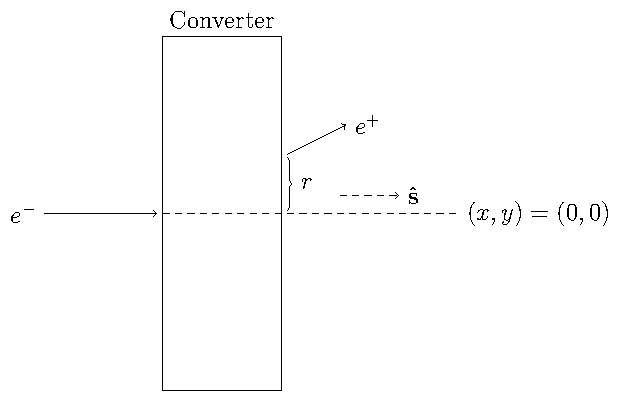
\includegraphics[width=0.6\textwidth]{coords1.pdf}
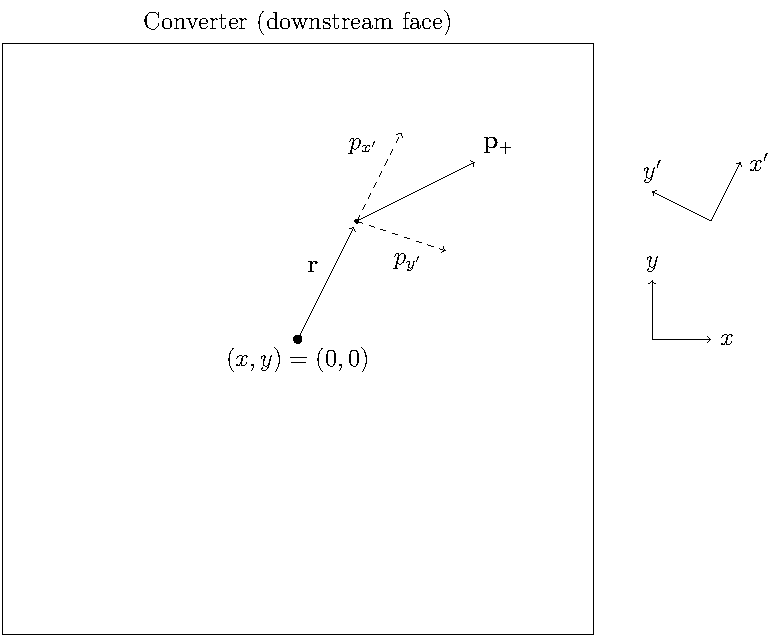
\includegraphics[width=0.8\textwidth]{coords2.pdf}
\caption{Coordinates used to describe the positrons exiting the converter.}
\end{figure}
The incoming electron beam is taken to be along the $z$-axis.
Outgoing positrons will exit the target with some displacement $r$ off of the $z$-axis, and have some energy $E_+$ and momentum $\pp_+$.
It is convenient to define a coordinate system $(x', y', z)$ with $\xx'$ pointing along the direction of $\rr$, and $\yy'$ taken perpendicular to $\xx'$ so that $(x', y', z)$ is a right-handed coordinate system.
This defines $p_x'$ and $p_y'$, the components of the outgoing positron momentum in the primed coordinate system.
We then define the "transverse momenta" $\frac{dx'}{ds}$ and $\frac{dy'}{ds}$ by
\begin{align}
\frac{dx'}{ds} & = \frac{p_x'}{p_z} \\
\frac{dy'}{ds} & = \frac{p_y'}{p_z}
\end{align}

\newpage

\section{The Model}
\label{s:model}

Given a positron converter of thickness $T$ and incoming electrons of energy $E_-$, we wish to predict $E_+$, $r$, $\frac{dx'}{ds}$, and $\frac{dy'}{ds}$ for the outgoing positrons.
We do this in two steps:
\begin{enumerate}
\item
First, we pull $E_+$ and $r$ from a two-dimensional probability distribution $P_1(E_+, r)$.
$P_1$ is determined by interpolation of the simulation data (see Section \ref{s:simulation}).

\item
For outgoing positrons of any given $(E_+, r)$, $\frac{dx'}{ds}$ and $\frac{dy'}{ds}$ appear to be distributed as
\begin{align}
P_2 \left( \dxds, \dyds ; E_+, r \right) & = A \frac{1 + \beta x}{1 + \alpha_x \left( \dxds - c_x \right)^2 + \alpha_y \left( \dyds \right)^2}.
\end{align}
Note that this functional form is empirically derived, and is not heavily motivated by the underlying physical processes that occur in the converter.
In out testing, we have found that this form does the best job of capturing the peak of the transverse momentum distribution, which is of greatest importance when the user cares about the positron capture efficiency of downstream linac elements.
%For users who care more about an accurate fit to the tails of the transverse momentum distribution, a bivariate normal distribution seems to be a better fit.

\end{enumerate}



\section{Obtaining the Model Coefficients}
\label{s:simulation}

Using the Geant4\cite{geant} software package developed at CERN, we have developed a program for simulating the production of positrons in the converter.
This program simulates the results of sending electrons of a fixed energy into a target of fixed thickness, and records the $E_+$, $r$, $\dxds$, and $\dyds$ values of the positrons that emerge at the downstream face of the converter.
The number of electrons used is determined dynamically so that good statistics on the properties of the produced positrons can be obtained.

With a large sample of positron data in hand, the program first bins the $E_+$ and $r$ data into a 2D histogram.
This binned data can then be interpolated to approximate the distribution of $E_+$ and $r$ values, $P_1(E_+, r)$.
After the $(E_+, r)$ bins are chosen, the $\dxds$ and $\dyds$ values for positrons in each bin are then themselves binned into 2D histograms.
We then fit the functional form described in Section \ref{s:model} to the binned $\dxds$, $\dyds$ data in each of the $(E_+, r)$ bins to obtain the fit parameters $A$, $\beta$, $\alpha_x$, $\alpha_y$ and $c_x$.
These fits gives us an approximation of $P_2 \left( \dxds, \dyds ; E_+, r \right)$.

Note that the distributions $P_1$ and $P_2$ will vary with incoming electron energy $E_-$ and target thickness $T$.
The program can be used to sample the behavior of the converter at various values of $E_-$ and $T$, and performs the above procedure once per $(E_-, T)$ pair.
\textit{Bmad} will then interpolate between the discrete set of $(E_-, T)$ values simulated to model the converter at any electron energy and target thickness in the range of interest.


\section{Input and Output of the Simulation}
\label{s:output}

To configure the simulation, the user edits the file \texttt{config.txt} in the same directory as the simulation program.
In this file, the user specifies the target material, a list of incoming electron energies $E_-$ to be tested, and a list of target thicknesses $T$ to be tested.
For each electron energy and target thickness pair, the program simulates the behavior of the converter for many incoming electrons, and outputs the following:
\begin{itemize}
\item
A table of the probability densities $P_1(E_+, r)$, automatically binned over the range of outgoing positron energies $E_+$ and radial displacements $r$ where positrons are produced.
This table is used by Bmad to approximate the probability distribution $P_1(E_+, r)$.

\item
Fits to the parameters $c_x$, $\alpha_x$, $\alpha_y$, and $\beta$ which describe the distribution of positron $\dxds$ and $\dyds$ values.
The program first bins the $\left( \dxds, \dyds \right)$ values of the positrons produced in each $(E_+, r)$ bin and fits the form of Equation 4 to this binned data.
This yields values for $c_x$, $\alpha_x$, $\alpha_y$, and $\beta$ in each $(E_+, r)$ bin.
The program then performs the following fits to $c_x(E_+, r)$, $\alpha_x(E_+, r)$, $\alpha_y(E_+, r)$, and $\beta(E_+, r)$:
\begin{itemize}
\item
At all values of $E_+$ and $r$,
\begin{align}
c_x(E_+, r) & = A_c E^{k_E} r^{k_r}
\end{align}

\item
For $\alpha_x$, $\alpha_y$, and $\beta$, their volitile behavior at low $E_+$ make obtaining a single 2D fit at all $E_+$ and $r$ values too difficult.
We therefore adopt a hybrid approach:
at low $E_+$, a series of 1D fits are performed at each value of $E_+$ to obtain $\alpha_x(r)$, $\alpha_y(r)$, and $\beta(r)$.
The values of $\alpha_x$, $\alpha_y$, and $\beta$ at values of $E_+$ in between the binned values are then obtained by linear interpolation.
At high $E_+$, a single 2D fit is performed to obtain $\alpha_x(E_+, r)$, $\alpha_y(E_+, r)$, and $\beta(E_+, r)$.

\item
For $\alpha_x$ and $\alpha_y$, the form
\begin{align}
\alpha_x(r), \alpha_y(r) = (a + br + cr^2 + dr^3) e^{-kr}
\end{align}
is used at low $E_+$, while the form
\begin{align}
\alpha_x(E_+, r), \alpha_y(E_+, r) & =
\frac{1}{E_+} e^{-(k_E E_+ + k_r r)}
(a_E + b_E E_+ + c_E E_+^2 + d_E E_+^3) \\
& \,\,\,\,\,\,\,\,\,\,\,\,\,\,\,\,\,\,\,\,\,\,\,\,\,\,\,\,\,\,\,\,\,\,\,\,\,\,\,\,\,\,\,\,\,\,\,\,\,\, (a_r + b_r r + c_r r^2 + d_r r^3)
\end{align}
is used at high $E_+$.

\item
For $\beta$, the form
\begin{align}
\beta(r) = a_0 + a_1 r + a_2 r^2 + a_3 r^3 + a_4 r^4
\end{align}
is used at low $E_+$, while the form
\begin{align}
\beta(E_+, r) = A_\beta E_+^{k_E} r^{k_r}
\end{align}
is used at high $E_+$.

\end{itemize}
These coeficients ($A_c, k_E, k_r$, etc) are obtained once for each electron energy and target thickness pair, and can be used to characterize the distribution $P_2 \left( \dxds, \dyds; E_+, r \right)$.

\end{itemize}

Using this output, \textit{Bmad} can simulate the converter's outgoing positrons with the probability distribution $P\left( E_+, r, \dxds, \dyds \right) = P_1(E_+, r) P_2 \left( \dxds, \dyds; E_+, r \right)$ at each of the discrete $E_-$ and $T$ values specified in the setup.
For electron energies at target thicknesses between the discrete set sampled by the Geant simulation, interpolation is used between the distributions at the four surrounding $(E_-, T)$ points sampled.



\printbibliography


\end{document}
